\documentclass{lab_sheet}
\usepackage{nccmath}
\usepackage{hyperref}
\newcommand{\figques}[3]{
   \begin{circuitikz}[scale=0.8,american]
      \draw
      (0,0) to[R,l=$1\Omega$] (4,0) to [L, l=$#1$ H] (8,0) to [C, *-*, l_=$#2$ F] (8,-4)
      (8,0) to [L, l=$#3$ H] (12,0)
      (0,0) to [esource,v_=$V_1$] (0,-4)
      (0,-4) to [short] (12,-4) to[R, l=$1\Omega$, v<=$V_2$] (12,0)
         ;
      \end{circuitikz}
}

\newcommand{\figafinal}{
   \begin{circuitikz}[scale=0.8,american]
      \draw
      (0,0) to[R,l=$200 \Omega$] (4,0) to [L, l=$20$ mH] (8,0) to [C, *-*, l_=$1\mu$F] (8,-4)
      (8,0) to [L, l=$20$ mH] (12,0)
      (0,0) to [esource,v_=$V_1$] (0,-4)
      (0,-4) to [short] (12,-4) to[R, l=$200\Omega$, v<=$V_2$] (12,0)
         ;
      \end{circuitikz}
}


\newcommand{\figbfinal}{
   \begin{circuitikz}[scale=0.8,american]
      \draw
      (0,0) to[R,l=$200 \Omega$] (4,0) to [L, l=$40.47$ mH] (8,0) to [C, *-*, l_=$0.49705\mu$F] (8,-4)
      (8,0) to [L, l=$40.47$ mH] (12,0)
      (0,0) to [esource,v_=$V_1$] (0,-4)
      (0,-4) to [short] (12,-4) to[R, l=$200\Omega$, v<=$V_2$] (12,0)
         ;
      \end{circuitikz}
}


\newcommand{\figcfinal}{
   \begin{circuitikz}[scale=0.8,american]
      \draw
      (0,0) to[R,l=$200 \Omega$] (4,0) to [L, l=$66.974$ mH] (8,0) to [C, *-*, l_=$0.3558\mu$F] (8,-4)
      (8,0) to [L, l=$66.974$ mH] (12,0)
      (0,0) to [esource,v_=$V_1$] (0,-4)
      (0,-4) to [short] (12,-4) to[R, l=$200\Omega$, v<=$V_2$] (12,0)
         ;
      \end{circuitikz}
}

\newcommand{\figdfinal}{
   \begin{circuitikz}[scale=0.8,american]
      \draw
      (0,0) to[R,l=$200 \Omega$] (4,0) to [L, l=$6.7484$ mH] (8,0) to [C, *-*, l_=$0.4852\mu$F] (8,-4)
      (8,0) to [L, l=$44.068$ mH] (12,0)
      (0,0) to [esource,v_=$V_1$] (0,-4)
      (0,-4) to [short] (12,-4) to[R, l=$200\Omega$, v<=$V_2$] (12,0)
         ;
      \end{circuitikz}
}


\newcommand{\proteusObservation}[4]{ 
\begin{figure}[H]
   \begin{minipage}[b]{0.60\linewidth}
     \centering
     \includegraphics[width=\linewidth]{../Figures/#1.PDF}
   \end{minipage}%
   \begin{minipage}[b]{0.40\linewidth}
     \centering
 \begin{tabular}[b]{|M{4cm}|M{1cm}|}
   \hline
   \multicolumn{2}{|c|}{Noted Values} \\
   \hline \hline
   Highest gain in pass band (in dB) & #2\\ \hline
   Half power frequency (in KHz) & #3\\ \hline
 \end{tabular}
 \end{minipage}
 \caption{Observation for #4}
 \label{fig:prot_obs__#1}
 \end{figure}
}

\newcommand{\proteusObservationBC}[6]{ 
\begin{figure}[H]
   \begin{minipage}[b]{0.60\linewidth}
     \centering
     \includegraphics[width=\linewidth]{../Figures/#1.PDF}
   \end{minipage}%
   \begin{minipage}[b]{0.40\linewidth}
     \centering
 \begin{tabular}[b]{|M{4cm}|M{1cm}|}
   \hline
   \multicolumn{2}{|c|}{Noted Values} \\
   \hline \hline
   Highest gain in pass band (in dB) & #2\\ \hline
   Half power frequency (in KHz) & #3\\ \hline
   Minimum gain due to ripple (in dB) & #4\\ \hline
   Ripple magnitude (in dB) & #5\\ \hline
 \end{tabular}
 \end{minipage}
 \caption{Observation for #6}
 \label{fig:prot_obs_bc_#1}
 \end{figure}
}


\begin{document}
    \titlePage{Comparison of Magnitude and Phase Response of Different Filters}{June 30, 2021}
    \pagenumbering{roman}
    \clearpage
    \tableofcontents
    \clearpage
    \phantomsection
    \addcontentsline{toc}{section}{\bfseries{List of figures}}
    \listoffigures
    \clearpage
    \phantomsection
    \addcontentsline{toc}{section}{\bfseries{List of Tables}}
    \listoftables
    \clearpage
    \pagenumbering{arabic}
    \section{Objectives}
    \begin{itemize}
        \item To design Butterworth, Chebyshev and Bessel filters.
        \item To observe and compare the magnitude and phase response of different filters.
    \end{itemize}

    \section{Background Theory}
    
    \subsection{Scaling}
    Impedance or Magnitude scaling is a process of scaling the impedances present in a network by a factor in such a way that the frequency response is unaltered. Similarly, frequency scaling is a process of shifting the frequency response of a network up or down the frequency axis in such a way that the impedance is unaltered. For magnitude scaling factor $K_m$ and frequency scaling factor $K_f$, the scaling equations for different filter network elements can be written as,

    \begin{equation}
        R_{new}=K_m.R_{old}
        \label{eqn:r_mag_freq}
     \end{equation}
     
     \begin{equation}
        L_{new}=\left(\frac{K_m}{K_f}\right)L_{old}
        \label{eqn:l_mag_freq}
     \end{equation}
     
     \begin{equation}
        C_{new}=\left(\frac{1}{K_m.K_f}\right)C_{old}
        \label{eqn:c_mag_freq}
     \end{equation}

     \subsection{Approximation Methods}
   To realize ideal filters, infinite number of components are required, which makes it practically unattainable. Hence, we need approximation methods for realizing practical filters. 
 The following requirements are to be fulfilled for low pass approximation:
 \begin{itemize}
    \item There should be small passband variation.
    \item There should be small passband attenuation and large stopband attenuation.
    \item It should have low transition band ratio.
    \item The network realization should be simple.
 \end{itemize}
 Since no network satisfies all the points, while designing, we trade off between circuit complexity and response.
     \subsubsection{Butterworth Filter}
     Butterworth filter has ideally flat passband such that for a filter with half power frequency of $\omega_0$, the frequency response is given by,
     \begin{equation}
        |T(jw)|^2=\frac{1}{1+\left(\frac{\omega}{\omega_0}\right)^{2n}}
     \end{equation}
     The order $n$ of the butterworth filter is given as,
     \begin{equation}
        n=\frac{\log\left(\frac{10^{\alpha_{min}/10}-1}{10^{\alpha_{max}/10}-1}\right)}{2\log\left(\frac{\omega_s}{\omega_p}\right)}
     \end{equation}

     \begin{figure}[H]
        \centering
        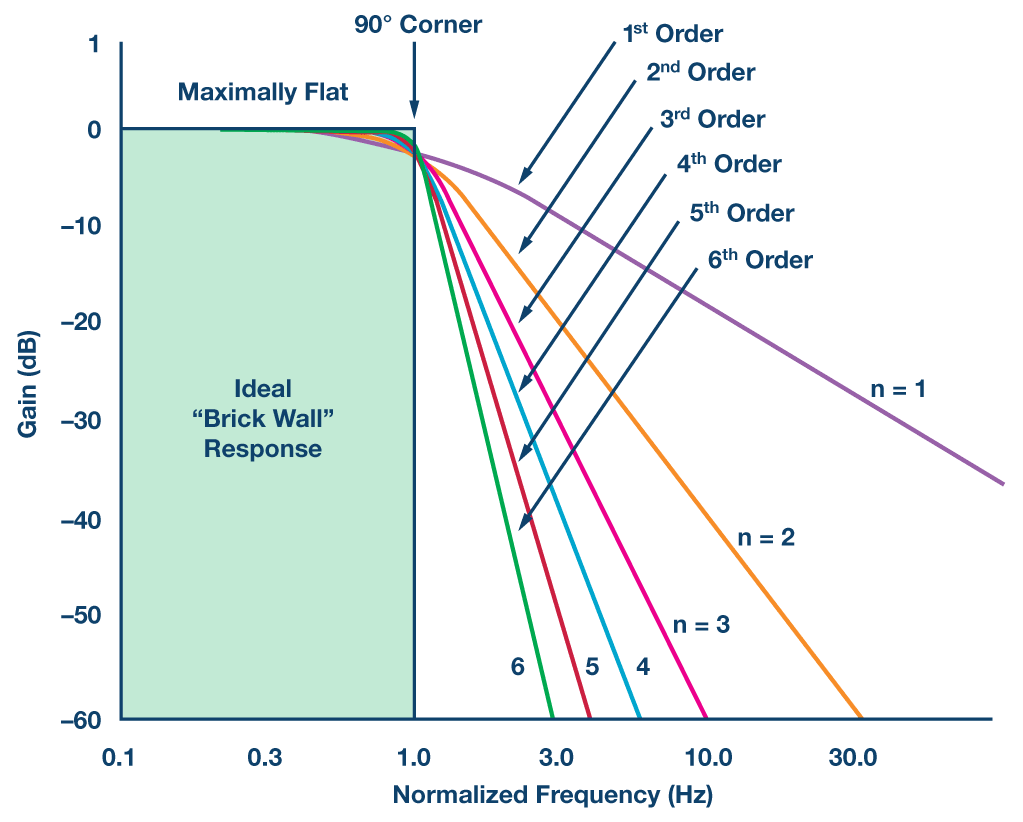
\includegraphics[width=0.6\linewidth]{../Figures/butter.png}
        \caption{Butterworth response for various ordered filters}
        \label{fig:butter}
     \end{figure}
     It's important to note that the passband is essentially flat, and the transition band of the butterworth filter is sharp with the increase in the order.
     The butterworth polynomial of degree n, which is used to determine the different poles of the filter is given as,
     \begin{equation}
        B_n(s)=\prod_k\left(s^2+2\cos(\psi_k)s+1\right)
     \end{equation}
     The reciprocal of $B_n(s)$ gives the transfer function of a $n^{th}$ order butterworth filter.
   \\
   To determine the values of $\psi_k$, the following rules are applied.
   \begin{itemize}
      \item If $n$ is odd, there is a pole at $\psi=0^{\circ}$, if $n$ is even there are poles at $\psi=\pm90^{\circ}/n$.
      \item Separation between poles is given by $\psi=180^{\circ}/n$
   \end{itemize}

     \subsubsection{Chebyshev Filter}
     Chebyshev filter has relatively sharper transition band and have ripple in either passband or the stop band. Depending on the presence of ripple, the chebyshev filter is categorized as chebyshev (type I) or inverse chebyshev (type II). For chebyshev polynomials, $C_n(\omega)$ and ripple factor $\epsilon$, the frequency response is given by,
     \begin{equation}
        |T(jw)|^2=\frac{1}{1+\epsilon^2C_n^2(\omega)}
     \end{equation}
     The chebyshev polynomials are defined as,
\begin{equation}
  C_n(\omega)= \begin{cases}
     \cos(n\cos^{-1}\omega),\quad\quad 0\leq\omega\leq 1\\
     \cosh(n\cosh^{-1}\omega),\quad\quad \omega\geq 1
      \end{cases}
\end{equation}
The relation between passband attenuation $\alpha_{max}$ and ripple factor $\epsilon$ is given as,
\begin{equation}
   \alpha_{max}=10\log(1+\epsilon^2)
\end{equation}
The chebyshev lowpass filter is characterized by, maximum attenuation in the passband $(\alpha_{max})$, minimum attenuation in the passband $(\alpha_{min})$, and stopband frequency $(\omega_s)$. For passband frequency $(\omega_p)=1$ rad/s, the order $n$ is calculated as,
\begin{equation}
   n=\frac{\cosh^{-1}\left(\sqrt{\frac{10^{\alpha_{max}/10}-1}{10^{\alpha_{min}/10}-1}}\right)}{\cosh^{-1}\omega_s}
\end{equation}
\begin{figure}[H]
   \centering
   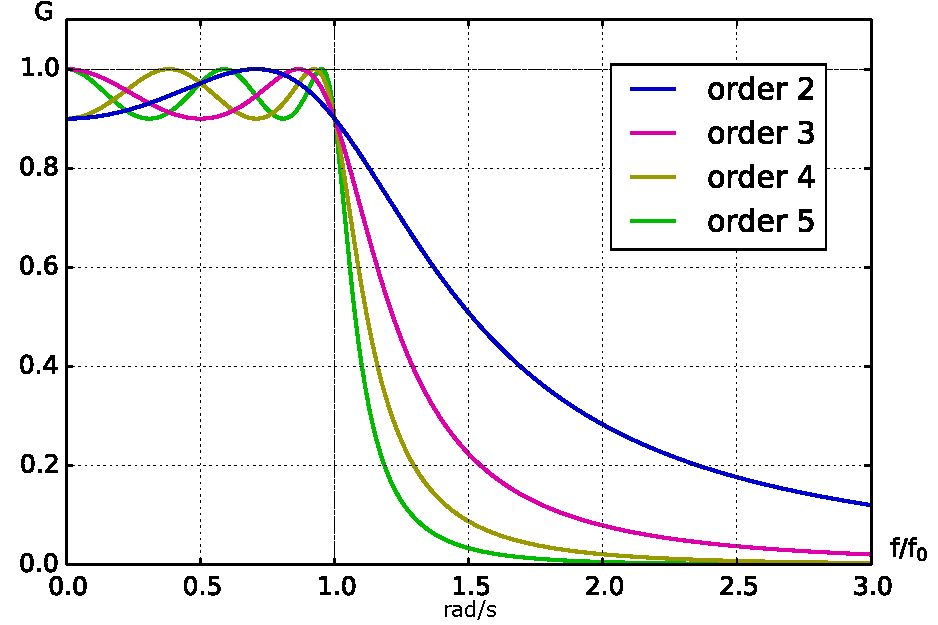
\includegraphics[width=0.7\linewidth]{../Figures/chebyshev.pdf}
   \caption{Chebyshev response for various ordered filters}
        \label{fig:chebyshev}
\end{figure}
The 3 dB frequency $\omega_c$ for chebyshev filter, is given as,
\begin{equation}
   \omega_c=\cosh\left(\frac{1}{n}\cosh^{-1}\frac{1}{\epsilon}\right)
\end{equation}
Similarly, the order $n$ for inverse chebyshev filter is calculated as,
\begin{equation}
   n=\frac{\cosh^{-1}\left(\sqrt{\frac{10^{\alpha_{min}/10}-1}{10^{\alpha_{max}/10}-1}}\right)}{\cosh^{-1}(\frac{1}{\omega_p})}
\end{equation}

\begin{figure}[H]
   \centering
   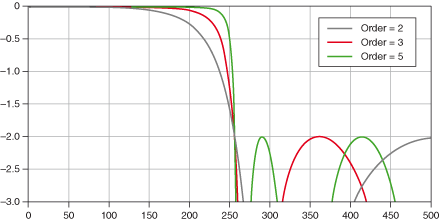
\includegraphics[width=0.8\linewidth]{../Figures/inverse.png}
   \caption{Inverse chebyshev response for various ordered filters}
        \label{fig:inverse}
\end{figure}
\subsubsection{Bessel Filter}
Bessel filter has somewhat of a linear phase response, so is used as a delay filter. It has the use-case of preserving the signal in the passband. For reverse bessel polynomial of degree $n$, $(\theta_n)$, the general form of a bessel filter is given as,
\begin{equation}
   T_n(s)=\frac{\theta_n(0)}{\theta_n(\frac{s}{\omega_0})}
\end{equation}

\begin{figure}[H]
   \centering
   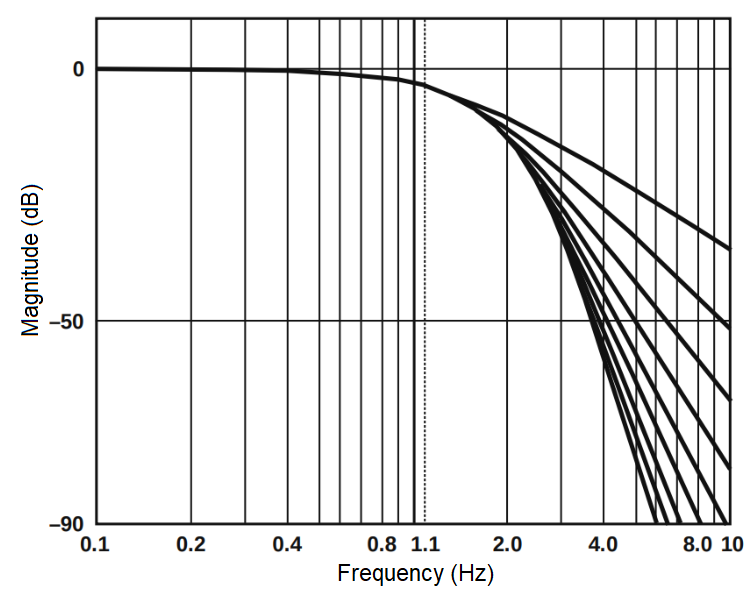
\includegraphics[width=0.5\linewidth]{../Figures/bessel.png}
   \caption{Bessel response for various ordered filters}
        \label{fig:bessel}
\end{figure}

\begin{figure}[H]
   \centering
   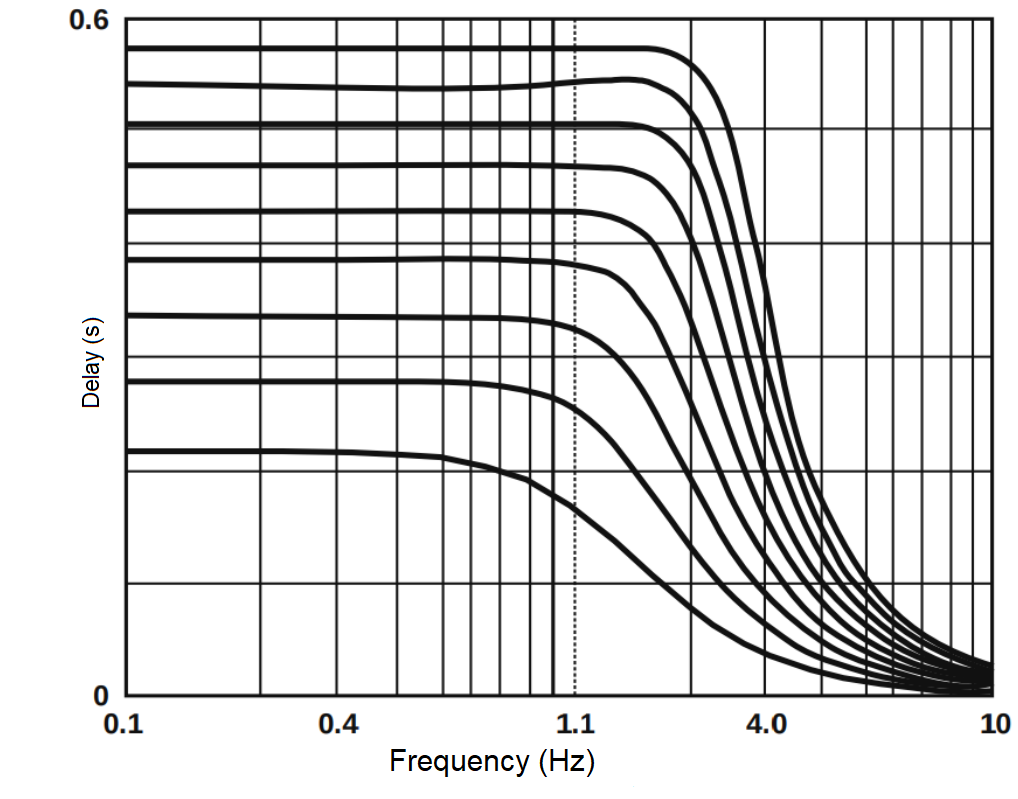
\includegraphics[width=0.5\linewidth]{../Figures/delay.png}
   \caption{Group delay of bessel filter for various ordered filters}
   \label{fig:delay}
\end{figure}
     \section{Exercises}
     \problem{The circuit given in figure \ref{fig:ques_a} below is a Butterworth low-pass filter having half power frequency of 1 rad/sec. From this circuit design a lowpass filter having half power frequency of 10000 rad/sec and practically realizable elements. Realize the circuit, observe and plot the magnitude as well as phase response. Also show the highest gain in dB and half power frequency in your plot. Observe the output in the oscilloscope when a square wave of 100 Hz is applied at input. Observe the output by increasing frequency upto 5 KHz. Comment on the result. Typically note down the output when the square wave around 1.6 KHz is applied at input.}

     \begin{figure}[H]
        \centering
        \figques{1}{2}{1}
        \caption{Third order butterworth filter}
        \label{fig:ques_a}
     \end{figure}

     Here,
\begin{fleqn}[\parindent]
   \begin{equation*}
      \begin{split}
         &\text{Half power frequency of given normalized filter } (\omega)=1 \text{ rad/s}\\
         &\text{Required half power frequency }(\Omega)=10000 \text{ rad/s} \\
         &\text{Frequency scaling factor }(K_f)=\frac{\Omega}{\omega}=10000
         \end{split}
      \end{equation*}
\end{fleqn}

To make the values of the elements practically realizable, we use a value of any element as desired and back-calculate the value of magnitude scaling factor $(K_m)$ using corresponding scaling equation. For this problem, let us assume that we require the final value of resistance in the circuit to be 200 $\Omega$.
\begin{fleqn}[\parindent]
   \begin{equation*}
      \begin{split}
         &\text{Required value of resistance } (R_{new})=200\Omega\\
         &\text{Old value of resistance }(R_{old})=1 \Omega 
      \end{split}
      \end{equation*}
\end{fleqn}
\begin{fleqn}[\parindent]
   \begin{equation*}
      \begin{split}
         &R_{new}={K_m}.R_{old}\\
         &\Rightarrow K_m = \frac{R_{new}}{R_{old}} = \frac{200}{1}=200 
      \end{split}
      \end{equation*}
\end{fleqn}
From these scaling factors we can calculate the new values of the inductor and capacitor from $L_{old}=1$ H and $C_{old}=2$ F using Equation~\ref{eqn:l_mag_freq} and \ref{eqn:c_mag_freq},
\begin{fleqn}[\parindent]
   \begin{equation*}
      \begin{split}
         &L_{new}=\left(\frac{K_m}{K_f}\right)L_{old}=\left(\frac{200}{10000}\right)1=20 \text{ mH}\\
         &C_{new}=\left(\frac{1}{K_m.K_f}\right)C_{old}=\left(\frac{1}{200\times10000}\right)2=1 \mu\text{F}
      \end{split}
      \end{equation*}
\end{fleqn}

\begin{figure}[H]
   \centering
   \figafinal
   \caption{Final circuit for low pass filter designed in Problem 1}
   \label{fig:figa}
\end{figure}

\begin{figure}[H]
   \centering
   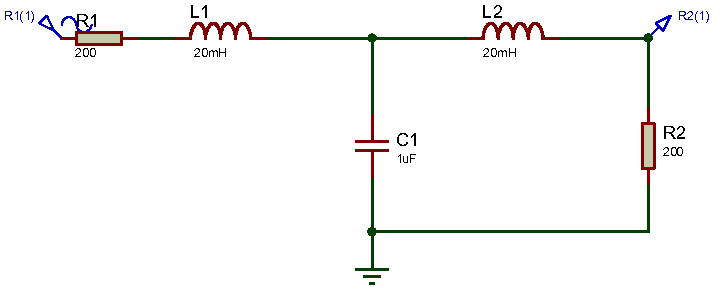
\includegraphics{../Figures/ckt_a}
   \caption{Proteus circuit for low pass filter designed in Problem 1}
   \label{fig:protA}
\end{figure}

\proteusObservation{protA}{-6.02}{1.59}{low pass filter designed in Problem 1}
As seen in Figure~\ref{fig:prot_obs__protA} ripples aren't present in passband, and there is a gradual transition between passband and stopband. These points can be used to characterize the filter as a butterworth filter.
\begin{figure}[H]
   \centering
   \begin{subfigure}{0.49\textwidth}
      \centering
   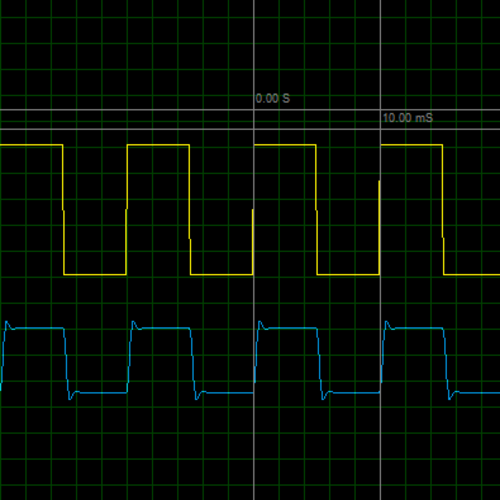
\includegraphics[width=0.9\linewidth]{../Figures/osc_a_1.png}
   \caption{When square wave of 100 Hz is applied}
   \end{subfigure}~
   \begin{subfigure}{0.49\textwidth}
      \centering
      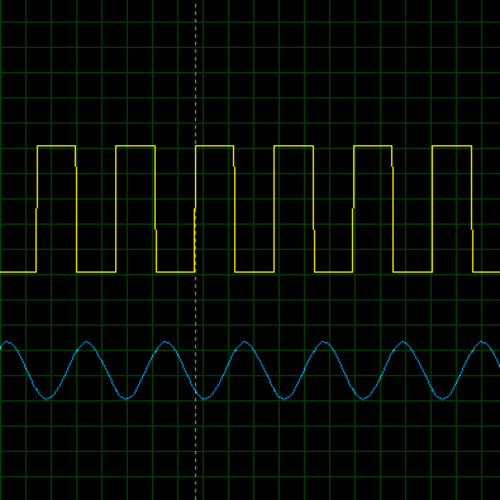
\includegraphics[width=0.9\linewidth]{../Figures/osc_a_3.png}
      \caption{When square wave of 1.6 KHz is applied}
      \end{subfigure}
      \caption{Observation for application of square wave to circuit shown in Figure \ref{fig:protA}}
   \label{fig:osc_a}
\end{figure}

\begin{figure}[H]
   \ContinuedFloat
   \centering
   \begin{subfigure}{0.49\textwidth}
      \centering
   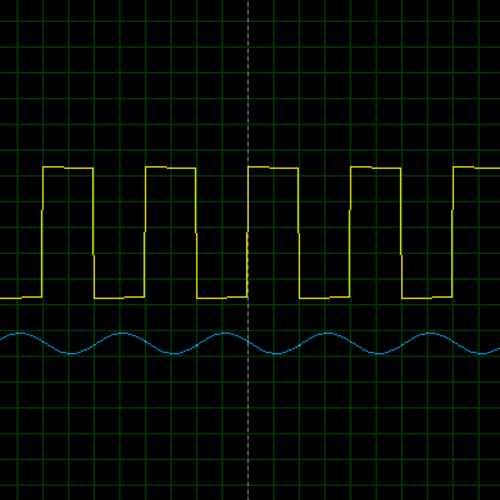
\includegraphics[width=0.9\linewidth]{../Figures/osc_a_4.png}
   \caption{When square wave of 2.5 KHz is applied}
   \end{subfigure}~
   \begin{subfigure}{0.49\textwidth}
      \centering
   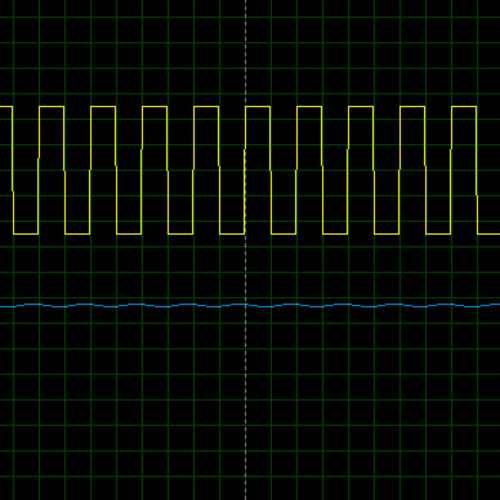
\includegraphics[width=0.9\linewidth]{../Figures/osc_a_2.png}
   \caption{When square wave of 5 KHz is applied}
   \end{subfigure}~
      \caption*{Figure~\ref{fig:osc_a}: Observation for application of square wave to circuit shown in Figure \ref{fig:protA} (continued)}
\end{figure}
Figure~\ref{fig:osc_a} shows the observation of oscilloscope when a square wave is applied to the designed low pass circuit. For low frequency of 100 Hz, attenuation and spikes near the transition is visible.  This is because of the attenuation, which causes gradual low state-high state transition. However, when the frequency of the square wave is at 1.6 KHz (half power frequency of the filter), a sine wave is seen at the output. For 2.5 KHz frequency, the higher components of the square wave are filtered leaving behind low frequency and dc components. At 5 KHz, much smoother output is obtained with minimum spikes.

     \problem{The circuit given in figure \ref{fig:ques_b} below is a low-pass Chebyshev filter having passband frequency of 1 rad/sec and attenuation of 1dB. From this circuit design a lowpass filter having passband frequency of 10000 rad/sec and practically realizable elements. Realize the circuit, observe and plot the magnitude as well as phase response. Also show the highest gain in dB and half power frequency in your plot. Note down the ripple within the entire passband. Observe the output in oscilloscope when square wave of 100 Hz is applied at input. Observe the output by increasing frequency upto 5 KHz. Comment on the result. Typically note down the output when square wave around 1.6 KHz is applied at input.}
 
     \begin{figure}[H]
      \centering
      \figques{2.0236}{0.9941}{2.0236}
      \caption{Chebyshev lowpass filter (1 dB ripple)}
      \label{fig:ques_b}
   \end{figure}

   Here,
   \begin{fleqn}[\parindent]
      \begin{equation*}
         \begin{split}
            &\text{Half power frequency of given normalized filter } (\omega)=1 \text{ rad/s}\\
            &\text{Required half power frequency }(\Omega)=10000 \text{ rad/s} \\
            &\text{Frequency scaling factor }(K_f)=\frac{\Omega}{\omega}=10000
            \end{split}
         \end{equation*}
   \end{fleqn}
   
   To make the values of the elements practically realizable, we use a value of any element as desired and back-calculate the value of magnitude scaling factor $(K_m)$ using corresponding scaling equation. For this problem, let us assume that we require the final value of resistance in the circuit to be 200 $\Omega$.
   \begin{fleqn}[\parindent]
      \begin{equation*}
         \begin{split}
            &\text{Required value of resistance } (R_{new})=200\Omega\\
            &\text{Old value of resistance }(R_{old})=1 \Omega 
         \end{split}
         \end{equation*}
   \end{fleqn}
   \begin{fleqn}[\parindent]
      \begin{equation*}
         \begin{split}
            &R_{new}={K_m}.R_{old}\\
            &\Rightarrow K_m = \frac{R_{new}}{R_{old}} = \frac{200}{1}=200 
         \end{split}
         \end{equation*}
   \end{fleqn}
   From these scaling factors we can calculate the new values of the inductor and capacitor from $L_{old}=2.0236$ H and $C_{old}=0.9941$ F using Equation~\ref{eqn:l_mag_freq} and \ref{eqn:c_mag_freq},
   \begin{fleqn}[\parindent]
      \begin{equation*}
         \begin{split}
            &L_{new}=\left(\frac{K_m}{K_f}\right)L_{old}=\left(\frac{200}{10000}\right)2.0236=40.47 \text{ mH}\\
            &C_{new}=\left(\frac{1}{K_m.K_f}\right)C_{old}=\left(\frac{1}{200\times10000}\right)0.9941=0.49705 \mu\text{F}
         \end{split}
         \end{equation*}
   \end{fleqn}
    
     
\begin{figure}[H]
   \centering
   \figbfinal
   \caption{Final circuit for low pass filter designed in Problem 2}
   \label{fig:figb}
\end{figure}

\begin{figure}[H]
   \centering
   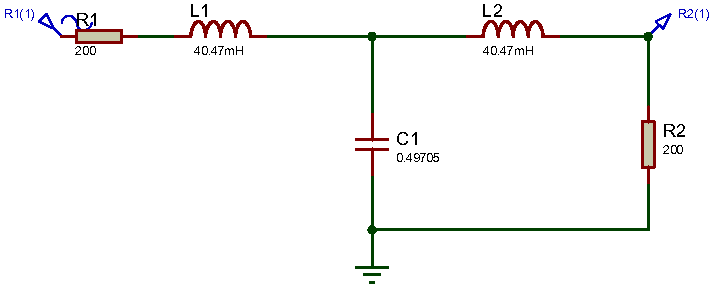
\includegraphics{../Figures/ckt_b}
   \caption{Proteus circuit for low pass filter designed in Problem 2}
   \label{fig:protB}
\end{figure}

\proteusObservationBC{protB}{-6.02}{1.72}{-7.02}{1}{low pass filter designed in Problem 2}

As seen in Figure~\ref{fig:prot_obs_bc_protB} ripple is present in passband. As stated in the observation table, the minimum ripple magnitude was found to be -7.02 dB, which means 1 dB ripple. These points can be used to characterize the filter as a chebyshev filter with 1 dB ripple.

\begin{figure}[H]
   \centering
   \begin{subfigure}{0.49\textwidth}
      \centering
   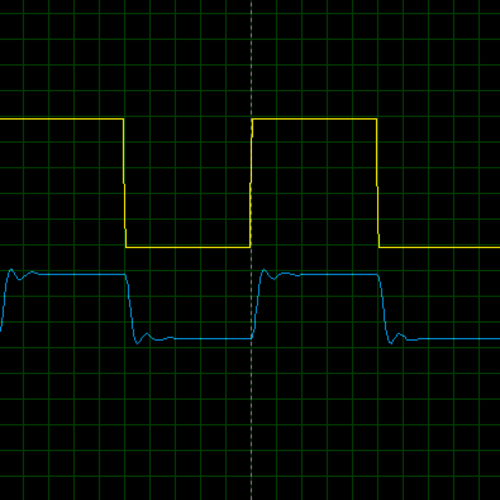
\includegraphics[width=0.9\linewidth]{../Figures/osc_b_1.png}
   \caption{When square wave of 100 Hz is applied}
   \end{subfigure}~
   \begin{subfigure}{0.49\textwidth}
      \centering
      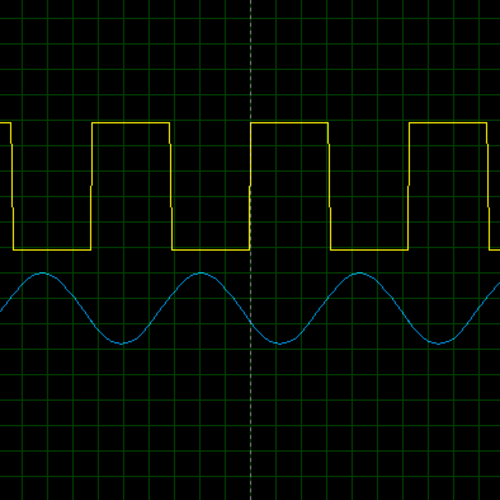
\includegraphics[width=0.9\linewidth]{../Figures/osc_b_2.png}
      \caption{When square wave of 1.6 KHz is applied}
      \end{subfigure}
      \caption{Observation for application of square wave to circuit shown in Figure \ref{fig:protB}}
   \label{fig:osc_b}
\end{figure}

\begin{figure}[H]
   \ContinuedFloat
   \centering
   \begin{subfigure}{0.49\textwidth}
      \centering
   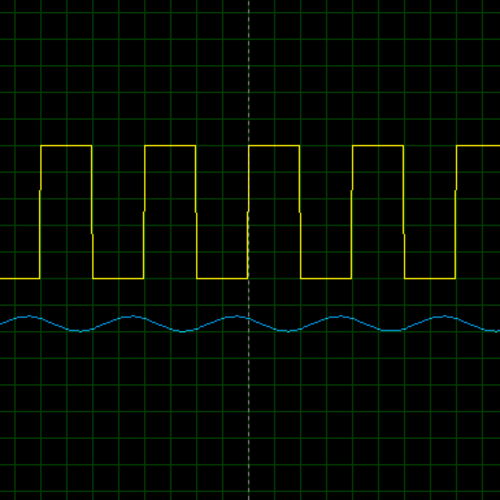
\includegraphics[width=0.9\linewidth]{../Figures/osc_b_4.png}
   \caption{When square wave of 2.5 KHz is applied}
   \end{subfigure}~
   \begin{subfigure}{0.49\textwidth}
      \centering
   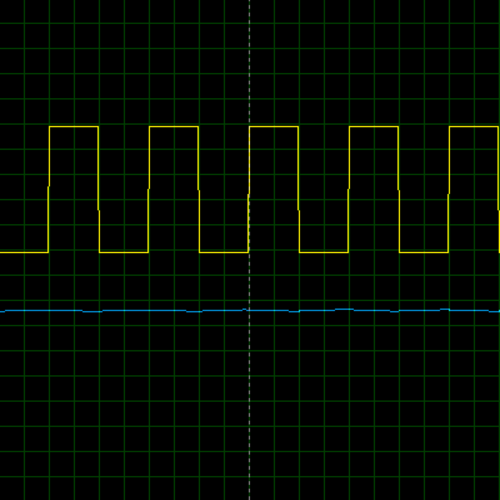
\includegraphics[width=0.9\linewidth]{../Figures/osc_b_3.png}
   \caption{When square wave of 5 KHz is applied}
   \end{subfigure}~
      \caption*{Figure~\ref{fig:osc_b}: Observation for application of square wave to circuit shown in Figure \ref{fig:protB} (continued)}
\end{figure}

Figure~\ref{fig:osc_b} shows the observation of oscilloscope when a square wave is applied to the designed low pass circuit. For low frequency of 100 Hz, attenuation and spikes near the transition is visible.  This is because of the ripple present in the passband of the filter response, and a resistive network. However, when the frequency of the square wave is at 1.6 KHz (half power frequency of the filter), a sine wave is seen at the output which is at $180^{\circ}$ phase difference from the original square wave. For 2.5 KHz frequency, the higher components of the square wave are filtered leaving behind low frequency and dc components. At 5 KHz, much smoother output is obtained.

   \problem{Let us modify the elements as shown in figure \ref{fig:ques_c} below to have the Chebyshev lowpass filter with 3 dB ripple. From this circuit design a lowpass filter having passband frequency of 10000 rad/sec and practically realizable elements. Realize the circuit, observe and plot the magnitude as well as phase response. Also show the highest gain in dB and half power frequency in your plot. Note down the ripple within the entire passband. Compare the response with that of problem 2.}

   \begin{figure}[H]
      \centering
      \figques{3.3487}{0.7117}{3.3487}
      \caption{Chebyshev lowpass filter (3 dB ripple)}
      \label{fig:ques_c}
   \end{figure}

   Here,
   \begin{fleqn}[\parindent]
      \begin{equation*}
         \begin{split}
            &\text{Half power frequency of given normalized filter } (\omega)=1 \text{ rad/s}\\
            &\text{Required half power frequency }(\Omega)=10000 \text{ rad/s} \\
            &\text{Frequency scaling factor }(K_f)=\frac{\Omega}{\omega}=10000
            \end{split}
         \end{equation*}
   \end{fleqn}
   
   To make the values of the elements practically realizable, we use a value of any element as desired and back-calculate the value of magnitude scaling factor $(K_m)$ using corresponding scaling equation. For this problem, let us assume that we require the final value of resistance in the circuit to be 200 $\Omega$.
   \begin{fleqn}[\parindent]
      \begin{equation*}
         \begin{split}
            &\text{Required value of resistance } (R_{new})=200\Omega\\
            &\text{Old value of resistance }(R_{old})=1 \Omega 
         \end{split}
         \end{equation*}
   \end{fleqn}
   \begin{fleqn}[\parindent]
      \begin{equation*}
         \begin{split}
            &R_{new}={K_m}.R_{old}\\
            &\Rightarrow K_m = \frac{R_{new}}{R_{old}} = \frac{200}{1}=200 
         \end{split}
         \end{equation*}
   \end{fleqn}
   From these scaling factors we can calculate the new values of the inductor and capacitor from $L_{old}=3.3487$ H and $C_{old}=0.7117$ F using Equation~\ref{eqn:l_mag_freq} and \ref{eqn:c_mag_freq},
   \begin{fleqn}[\parindent]
      \begin{equation*}
         \begin{split}
            &L_{new}=\left(\frac{K_m}{K_f}\right)L_{old}=\left(\frac{200}{10000}\right)3.3487=66.974 \text{ mH}\\
            &C_{new}=\left(\frac{1}{K_m.K_f}\right)C_{old}=\left(\frac{1}{200\times10000}\right)0.7117=0.3558 \mu\text{F}
         \end{split}
         \end{equation*}
   \end{fleqn}
   
\begin{figure}[H]
 \centering
 \figcfinal
 \caption{Final circuit for low pass filter designed in Problem 3}
 \label{fig:figc}
\end{figure}

\begin{figure}[H]
 \centering
 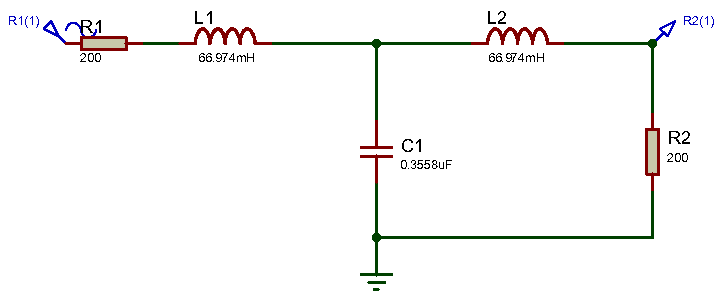
\includegraphics{../Figures/ckt_c}
 \caption{Proteus circuit for low pass filter designed in Problem 3}
 \label{fig:protC}
\end{figure}

\proteusObservationBC{protC}{-6.02}{1.59}{-9.02}{3}{low pass filter designed in Problem 3}
As seen in Figure~\ref{fig:prot_obs_bc_protC} ripple is present in passband. As stated in the observation table, the minimum ripple magnitude was found to be -9.02 dB, which means 3 dB ripple. These points can be used to characterize the filter as a chebyshev filter with 3 dB ripple. An important thing to note is that the besides having larger ripple in passband, the response for the designed low pass filter in Problem 3 has a sharper transition than that designed in Problem 2. 
   \problem{The circuit given in figure \ref{fig:ques_d} below is a low-pass Bessel filter with normalized frequency. From this circuit design a lowpass filter for the frequency of 10000 rad/sec. All the elements of your final design should be practically realizable. Realize the circuit, observe and plot the magnitude as well as phase response. Also show the highest gain in dB and half power frequency in your plot. Observe the output in oscilloscope when square wave of 100 Hz is applied at input. Observe the output by increasing frequency upto 5 KHz. Comment on the result. Typically note down the output when the square wave around 1.6 KHz is applied at input.}

   \begin{figure}[H]
      \centering
      \figques{0.337421}{0.970512}{2.203411}
      \caption{Bessel filter at normalized frequency}
      \label{fig:ques_d}
   \end{figure}

   
   Here,
   \begin{fleqn}[\parindent]
      \begin{equation*}
         \begin{split}
            &\text{Half power frequency of given normalized filter } (\omega)=1 \text{ rad/s}\\
            &\text{Required half power frequency }(\Omega)=10000 \text{ rad/s} \\
            &\text{Frequency scaling factor }(K_f)=\frac{\Omega}{\omega}=10000
            \end{split}
         \end{equation*}
   \end{fleqn}
   
   To make the values of the elements practically realizable, we use a value of any element as desired and back-calculate the value of magnitude scaling factor $(K_m)$ using corresponding scaling equation. For this problem, let us assume that we require the final value of resistance in the circuit to be 200 $\Omega$.
   \begin{fleqn}[\parindent]
      \begin{equation*}
         \begin{split}
            &\text{Required value of resistance } (R_{new})=200\Omega\\
            &\text{Old value of resistance }(R_{old})=1 \Omega 
         \end{split}
         \end{equation*}
   \end{fleqn}
   \begin{fleqn}[\parindent]
      \begin{equation*}
         \begin{split}
            &R_{new}={K_m}.R_{old}\\
            &\Rightarrow K_m = \frac{R_{new}}{R_{old}} = \frac{200}{1}=200 
         \end{split}
         \end{equation*}
   \end{fleqn}
   From these scaling factors we can calculate the new values of the inductor and capacitor from $L_{1old}=0.337421$ H, $L_{2old}=2.203411$ H and $C_{old}=0.9941$ F using Equation~\ref{eqn:l_mag_freq} and \ref{eqn:c_mag_freq},
   \begin{fleqn}[\parindent]
      \begin{equation*}
         \begin{split}
            &L_{1new}=\left(\frac{K_m}{K_f}\right)L_{1old}=\left(\frac{200}{10000}\right)0.337421=6.7484 \text{ mH}\\
            &L_{2new}=\left(\frac{K_m}{K_f}\right)L_{2old}=\left(\frac{200}{10000}\right)2.203411=44.068 \text{ mH}\\
            &C_{new}=\left(\frac{1}{K_m.K_f}\right)C_{old}=\left(\frac{1}{200\times10000}\right)0.970512=0.4852 \mu\text{F}
         \end{split}
         \end{equation*}
   \end{fleqn}
    
     
\begin{figure}[H]
   \centering
   \figdfinal
   \caption{Final circuit for low pass filter designed in Problem 4}
   \label{fig:figd}
\end{figure}

\begin{figure}[H]
   \centering
   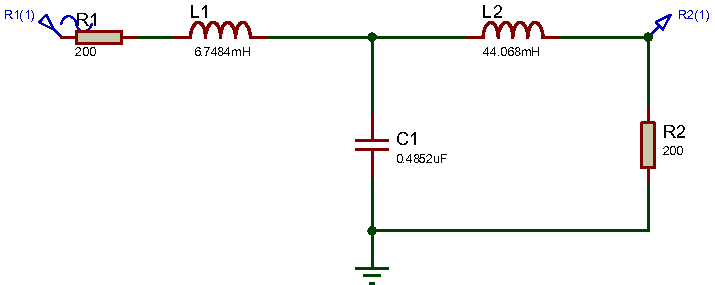
\includegraphics{../Figures/ckt_d}
   \caption{Proteus circuit for low pass filter designed in Problem 4}
   \label{fig:protD}
\end{figure}

\proteusObservation{protD}{-6.02}{1.59}{low pass filter designed in Problem 4}

As seen in Figure~\ref{fig:prot_obs__protD} ripples aren't present in passband. Similarly, the transition between the passband and stopband is much smoother and slower than that designed in Problem 1 (Butterworth filter). Another key characteristic is that the phase response of bessel filter seems to be almost linear in the passband. 

\begin{figure}[H]
   \centering
   \begin{subfigure}{0.49\textwidth}
      \centering
   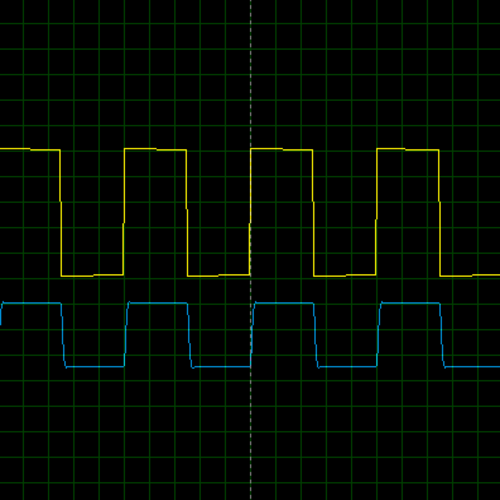
\includegraphics[width=0.9\linewidth]{../Figures/osc_d_1.png}
   \caption{When square wave of 100 Hz is applied}
   \end{subfigure}~
   \begin{subfigure}{0.49\textwidth}
      \centering
      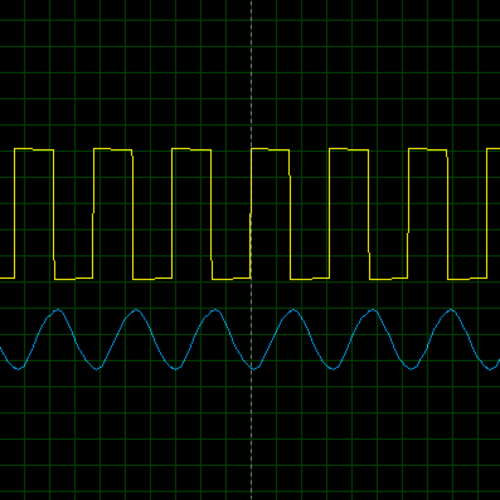
\includegraphics[width=0.9\linewidth]{../Figures/osc_d_2.png}
      \caption{When square wave of 1.6 KHz is applied}
      \end{subfigure}
      \caption{Observation for application of square wave to circuit shown in Figure \ref{fig:protD}}
   \label{fig:osc_d}
\end{figure}

\begin{figure}[H]
   \ContinuedFloat
   \centering
   \begin{subfigure}{0.49\textwidth}
      \centering
   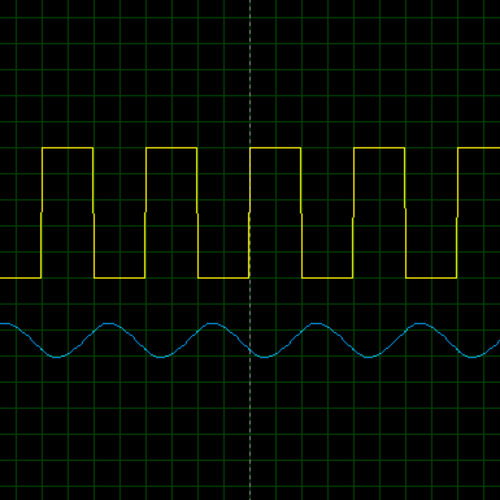
\includegraphics[width=0.9\linewidth]{../Figures/osc_d_4.png}
   \caption{When square wave of 2.5 KHz is applied}
   \end{subfigure}~
   \begin{subfigure}{0.49\textwidth}
      \centering
   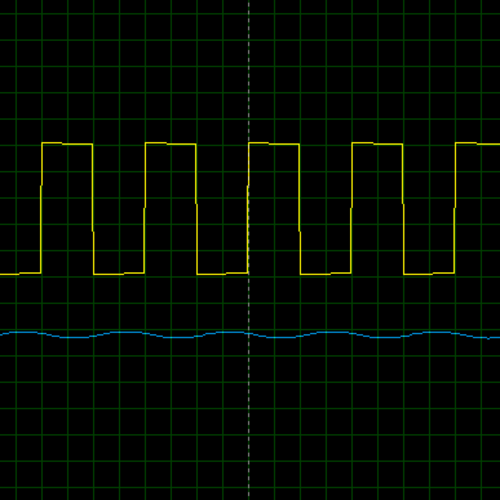
\includegraphics[width=0.9\linewidth]{../Figures/osc_d_3.png}
   \caption{When square wave of 5 KHz is applied}
   \end{subfigure}
      \caption*{Figure~\ref{fig:osc_d}: Observation for application of square wave to circuit shown in Figure \ref{fig:protD} (continued)}
\end{figure}

Figure~\ref{fig:osc_d} shows the observation of oscilloscope when a square wave is applied to the designed low pass circuit. For low frequency of 100 Hz, output shape is somewhat identical to the input, with almost identical phase and half amplitude.  Similarly, when the frequency of the square wave is at 1.6 KHz (half power frequency of the filter), a sine wave is seen at the output which is at some phase difference from the original square wave. For 2.5 KHz frequency, the higher components of the square wave are filtered leaving behind low frequency and dc components, which is why the output isn't a ideal sine wave. Ripples are visible with larger magnitude than that seen in Problem 1. This is due to lower attenuation for higher frequencies.  At 5 KHz, much smoother and somewhat constant output is obtained. However, the ripples are visible in larger magnitude than that in Problem 1 due to the same fact as stated earlier.

\section{Discussion and Conclusion}
In this lab experiment, we visualized the different magnitude and phase responses of butterworth, chebyshev (1 dB and 3 dB ripple) and bessel filters. Based on the observations, we can summarize the observation as,
\begin{table}[H]
   \centering
   \begin{tabular}{|c|M{3.5cm}|M{6.5cm}|}
   \hline
   \textbf{Filter Type}             & \textbf{Ripple in passband}           & \textbf{Transition zone}                                                                           \\ \hline\hline
   Butterworth              & No (Maximally flat passband)  & Steeper than Bessel filter, but not as good as Chebyshev                                  \\ \hline
   Chebyshev (1 dB ripple) & Yes (1 dB ripple in passband) & Steeper than Butterworth filter and Bessel filter but slower than chebyshev (3 dB ripple) \\ \hline
   Chebyshev (3 dB ripple) & Yes (3 dB ripple in passband) & Steeper than Butterworth filter, Bessel filter and chebyshev (1 dB ripple)                \\ \hline
   Bessel                  & No (Flat passband)            & Slower than Butterworth filter and Chebyshev filter                                       \\ \hline
   \end{tabular}
   \caption{Comparison summary between the given filters}
   \label{tbl:comp}
\end{table}
It was also noted that for application of square wave of same frequencies to various designed filters in the given problems, varying effects were seen after filtering. \\
Hence, the objectives of the lab were fulfilled with the understanding of the necessity of the mentioned topics.
\end{document}